% !TEX TS-program = XeLaTeX
% use the following command: 
% all document files must be coded in UTF-8
\documentclass{textolivre}
% for anonymous submission
%\documentclass[anonymous]{textolivre}
% to create HTML use 
%\documentclass{textolivre-html}
% See more information on the repository: https://github.com/leolca/textolivre

% Metadata
\begin{filecontents*}[overwrite]{article.xmpdata}
    \Title{Tecnología y abstracción: desarrollo de habilidades complejas a través de vídeo juegos}
    \Author{Andrea del Carmen Figueroa Vargas \sep Margarita Ercilia Aravena Gaete \sep María Natalia Campos Soto \sep David Ruete Zuñiga}
    \Language{es}
    \Keywords{pensamiento superior \sep habilidades cognitivas \sep abstracción \sep video juegos \sep modelos proyectivos \sep tecnología}
    \Journaltitle{Texto Livre}
    \Journalnumber{1983-3652}
    \Volume{14}
    \Issue{2}
    \Firstpage{1}
    \Lastpage{32}
    \Doi{10.35699/1983-3652.2021.29629}

    \setRGBcolorprofile{sRGB_IEC61966-2-1_black_scaled.icc}
            {sRGB_IEC61966-2-1_black_scaled}
            {sRGB IEC61966 v2.1 with black scaling}
            {http://www.color.org}
\end{filecontents*}

% used to create dummy text for the template file
\definecolor{dark-gray}{gray}{0.35} % color used to display dummy texts
\usepackage{lipsum}
\SetLipsumParListSurrounders{\colorlet{oldcolor}{.}\color{dark-gray}}{\color{oldcolor}}

% used here only to provide the XeLaTeX and BibTeX logos
\usepackage{hologo}

% used in this example to provide source code environment
%\crefname{lstlisting}{lista}{listas}
%\Crefname{lstlisting}{Lista}{Listas}
%\usepackage{listings}
%\renewcommand\lstlistingname{Lista}
%\lstset{language=bash,
        breaklines=true,
        basicstyle=\linespread{1}\small\ttfamily,
        numbers=none,xleftmargin=0.5cm,
        frame=none,
        framexleftmargin=0.5em,
        framexrightmargin=0.5em,
        showstringspaces=false,
        upquote=true,
        commentstyle=\color{gray},
        literate=%
           {á}{{\'a}}1 {é}{{\'e}}1 {í}{{\'i}}1 {ó}{{\'o}}1 {ú}{{\'u}}1 
           {à}{{\`a}}1 {è}{{\`e}}1 {ì}{{\`i}}1 {ò}{{\`o}}1 {ù}{{\`u}}1
           {ã}{{\~a}}1 {ẽ}{{\~e}}1 {ĩ}{{\~i}}1 {õ}{{\~o}}1 {ũ}{{\~u}}1
           {â}{{\^a}}1 {ê}{{\^e}}1 {î}{{\^i}}1 {ô}{{\^o}}1 {û}{{\^u}}1
           {ä}{{\"a}}1 {ë}{{\"e}}1 {ï}{{\"i}}1 {ö}{{\"o}}1 {ü}{{\"u}}1
           {Á}{{\'A}}1 {É}{{\'E}}1 {Í}{{\'I}}1 {Ó}{{\'O}}1 {Ú}{{\'U}}1
           {À}{{\`A}}1 {È}{{\`E}}1 {Ì}{{\`I}}1 {Ò}{{\`O}}1 {Ù}{{\`U}}1
           {Ã}{{\~A}}1 {Ẽ}{{\~E}}1 {Ũ}{{\~u}}1 {Õ}{{\~O}}1 {Ũ}{{\~U}}1
           {Â}{{\^A}}1 {Ê}{{\^E}}1 {Î}{{\^I}}1 {Ô}{{\^O}}1 {Û}{{\^U}}1
           {Ä}{{\"A}}1 {Ë}{{\"E}}1 {Ï}{{\"I}}1 {Ö}{{\"O}}1 {Ü}{{\"U}}1
           {ç}{{\c{c}}}1 {Ç}{{\c{C}}}1
}


\journalname{Texto Livre}
\thevolume{14}
\thenumber{2}
\theyear{2021}
\receiveddate{\DTMdisplaydate{2020}{12}{11}{-1}} % YYYY MM DD
\accepteddate{\DTMdisplaydate{2021}{02}{28}{-1}}
\publisheddate{\today}
% Corresponding author
\corrauthor{Andrea del Carmen Figueroa Vargas}
% DOI
\articledoi{10.35699/1983-3652.2021.33575}
% list of available sesscions in the journal: articles, dossier, reports, essays, reviews, interviews, editorial
\articlesessionname{dossier}
% Abbreviated author list for the running footer
\runningauthor{Figueroa Vargas}
\editorname{Anna Izabella Miranda Pereira}

\title{Tecnología y abstracción: desarrollo de habilidades complejas a través de vídeo juegos}
\othertitle{Tecnologia e abstração: desenvolvimento de habilidades complexas por meio de videogames}
\othertitle{Technology and abstraction: complex skills development through video games}
% if there is a third language title, add here:
%\othertitle{Artikelvorlage zur Einreichung beim Texto Livre Journal}

\author[1]{Andrea del Carmen Figueroa Vargas \orcid{0000-0002-6285-4373} \thanks{Email: \url{afigueroav@udla.cl}}}
\author[1]{Margarita Ercilia Aravena Gaete \orcid{0000-0003-3198-8384} \thanks{Email: \url{margarita.aravena.gaete@ed.udla.cl}}}
\author[2]{María Natalia Campos Soto \orcid{0000-0002-3361-2930} \thanks{Email: \url{ncampos@ugr.es}}}
\author[3]{David Ruete Zuñiga \orcid{0000-0002-7100-9737} \thanks{Email: \url{druete@unab.cl}}}

\affil[1]{Universidad de Las Américas, Facultad de Educación – Escuela de Educación Parvularia, Santiago, Región Metropolitana, Chile.}
\affil[2]{Universidad de Granada, Facultad de Ciencias de la Educación, Departamento de Didáctica y organización Escolar, Granada, España.}
\affil[3]{Universidad Andres Bello, Facultad de Ingeniería, Viña del mar, Región de Valparaíso, Chile.}

\addbibresource{article.bib}
% use biber instead of bibtex
% $ biber tl-article-template

% set language of the article
\setdefaultlanguage{spanish}
\setotherlanguage{portuguese}
\setotherlanguage{english}

% for spanish, use:
%\setdefaultlanguage{spanish}
\gappto\captionsspanish{\renewcommand{\tablename}{Tabla}} % use 'Tabla' instead of 'Cuadro'
\AfterEndPreamble{\crefname{table}{tabla}{tablas}\Crefname{table}{Tabla}{Tablas}}

% for languages that use special fonts, you must provide the typeface that will be used
% \setotherlanguage{arabic}
% \newfontfamily\arabicfont[Script=Arabic]{Amiri}
% \newfontfamily\arabicfontsf[Script=Arabic]{Amiri}
% \newfontfamily\arabicfonttt[Script=Arabic]{Amiri}
%
% in the article, to add arabic text use: \textlang{arabic}{ ... }

% to use emoticons in your manuscript
% https://stackoverflow.com/questions/190145/how-to-insert-emoticons-in-latex/57076064
% using font Symbola, which has full support
% the font may be downloaded at:
% https://dn-works.com/ufas/
% add to preamble:
% \newfontfamily\Symbola{Symbola}
% in the text use:
% {\Symbola }

% reference itens in a descriptive list using their labels instead of numbers
% insert the code below in the preambule:
\makeatletter
\let\orgdescriptionlabel\descriptionlabel
\renewcommand*{\descriptionlabel}[1]{%
  \let\orglabel\label
  \let\label\@gobble
  \phantomsection
  \edef\@currentlabel{#1\unskip}%
  \let\label\orglabel
  \orgdescriptionlabel{#1}%
}
\makeatother
%
% in your document, use as illustraded here:
%\begin{description}
%  \item[first\label{itm1}] this is only an example;
%  % ...  add more items
%\end{description}
 

% custom epigraph - BEGIN 
%%% https://tex.stackexchange.com/questions/193178/specific-epigraph-style
\usepackage{epigraph}
\renewcommand\textflush{flushright}
\makeatletter
\newlength\epitextskip
\pretocmd{\@epitext}{\em}{}{}
\apptocmd{\@epitext}{\em}{}{}
\patchcmd{\epigraph}{\@epitext{#1}\\}{\@epitext{#1}\\[\epitextskip]}{}{}
\makeatother
\setlength\epigraphrule{0pt}
\setlength\epitextskip{0.5ex}
\setlength\epigraphwidth{.7\textwidth}
% custom epigraph - END


% if you use multirows in a table, include the multirow package
\usepackage{multirow}


\begin{document}
\maketitle

\begin{polyabstract}
\begin{abstract}
El objetivo de este estudio es proponer modelos de aprendizaje de máquina supervisada  para predecir la capacidad de abstracción en los estudiantes, como mecanismo de alerta temprana, a través de la utilización de la tecnología y el uso del video juego. La metodología utilizada es mixta, con un diseño descriptivo y predictivo, se analizaron 118 tests aplicados a estudiantes chilenos de formación docente. Para ello, se correlacionaron las variables: edad, modalidad y semestre académico y se examinaron seis modelos predictivos. Los resultados evidencian tres hallazgos relevantes. En primer lugar, en la relación abstracción/edad, en las categorías Satisfactoria y No Abstracción, la distribución es homogénea en todas las edades. En segundo lugar, la relación abstracción/modalidad se evidencia que sigue un patrón del 50\% para todas las categorías de abstracción. En tercer lugar, la relación abstracción/semestre académico, se observa que en el séptimo semestre se concentra la mayor cantidad de estudiantes sin capacidad de abstracción. Se concluye que el nivel de abstracción es bajo,  evidenciándose que el 61,1\% de los estudiantes no tiene un nivel cognitivo superior. De los 6 modelos de aprendizaje de máquina supervisada, dos se sugieren para predecir una alerta temprana, árbol de decisión y bosque aleatorio que tienen una exactitud (Accuracy) del 100\%. Por lo tanto, mediante el uso de la tecnología y el video juego es posible afianzar el desarrollo de habilidades cognitivas superiores,  por medio de una serie de estrategias planificadas en tiempos de covid-19, concentradas en el primer y segundo semestre de formación.

\keywords{pensamiento superior \sep habilidades cognitivas \sep abstracción \sep video juegos \sep modelos proyectivos \sep tecnología}
\end{abstract}

\begin{portuguese} 
\begin{abstract}
O objetivo deste estudo é propor modelos de aprendizado de máquina supervisionado para predizer a capacidade de abstração em alunos, como mecanismo de alerta precoce, por meio do uso de tecnologia e de videogames. A metodologia utilizada é mista, com desenho descritivo e preditivo, analisando 118 testes aplicados a alunos chilenos de formação de professores. Para isso, as variáveis: idade, modalidade e semestre letivo foram correlacionadas e seis modelos preditivos foram examinados. Os resultados mostram três achados relevantes. Primeiro, na relação abstração/idade, nas categorias Satisfatório e Não Abstração, a distribuição é homogênea em todas as idades. Em segundo lugar, a relação abstração/modalidade evidencia que segue um padrão de 50\% para todas as categorias de abstração. Terceiro, na relação abstração/semestre letivo, observa-se que no sétimo semestre concentra-se o maior número de alunos sem capacidade de abstração. Conclui-se que o nível de abstração é baixo, mostrando que 61,1\% dos alunos não possuem um nível cognitivo superior. Dos 6 modelos de aprendizado de máquina supervisionados, dois são sugeridos para prever o aviso prévio, a árvore de decisão e a floresta aleatória com 100\% de precisão (Precisão). Portanto, por meio do uso de tecnologia e videogames, é possível fortalecer o desenvolvimento de habilidades cognitivas superiores, por meio de uma série de estratégias planejadas em tempos de COVID-19, concentradas no primeiro e no segundo semestres de treinamento.

\keywords{Pensamento superior \sep Habilidades cognitivas \sep Abstração \sep Videogames \sep Modelos projetivos \sep Tecnologia}
\end{abstract}
\end{portuguese}


\begin{english}
\begin{abstract}
This study aims to propose supervised machine learning models to predict the abstraction ability in students as an early warning mechanism through both the technology use and the video game use. The methodology used was mixed with a prescriptive and predictive design; 118 tests were carried out by Chilean pedagogy students. For analysis, several variables were correlated: age, modality, academic semester and six predictive models. The results show three relevant findings; First, regarding the relation abstraction/ age, in the Satisfactory and No abstraction, the distribution is homogeneous in every age. Second, the relationship abstraction/modality shows a 50\% pattern for all the abstraction categories. Third, the relation abstraction/academic semester shows that most students from the seventh semester have no capacity for abstraction. The study concludes the abstraction level is low, showing that 61,1\% of the students do not have a higher cognitive level. Two out of six of the supervised machine learning models are suggested to predict early warning, decision tree and random forest since they have a 100\% accuracy. Therefore, through the use of technology and the video game it is possible to ensure higher cognitive level development, by the use of several planned strategies in covid-19 times concentrated in the first two tears of pedagogy training.

\keywords{higher thinking \sep cognitive skill \sep abstraction \sep play games \sep projective models \sep technology}
\end{abstract}
\end{english}

% if there is another abstract, insert it here using the same scheme
\end{polyabstract}


\section{Introducción}\label{intro}
La utilización de la Tecnología para el desarrollo de habilidades cognitivas en los estudiantes tiene su génesis a partir de la convergencia de la psicología cognitiva y el uso y tratamiento pedagógico de las tecnologías asociadas a la Educación. En esta línea, varios autores \cite{escontrela2004, remolinacaviedes2014, gargallo2018} %(ESCONTRELA y STOJANOVIC, 2004; REMOLINA, 2014; GARGALLO; 2018)
han señalado ampliamente los beneficios de la Tecnología en planos de integración pedagógica siendo un recurso fundamental para favorecer el aprendizaje. Así emerge el concepto de aprendizaje basado en la tecnología \cite{ertmer2010} %(ERTMER Y OTTENBREIT-LEFTWICH, 2010)
para articular, distinguir y focalizar el propósito educativo en la acción docente y, con ello, desde la perspectiva del desarrollo de habilidades potenciar  habilidades complejas de pensamiento.

La utilización de videojuegos como estrategia para el desarrollo de habilidades cognitivas mediadas por la tecnología, se vuelve interesante de explorar por las potencialidades pedagógicas, especialmente, para el estudiantado de educación superior. En este marco, los videojuegos facilitan la complejización de una serie de habilidades que mediadas y organizadas pedagógicamente permiten facilitar el desarrollo de habilidades bajo un escenario cercano al estudiantado que al incluir códigos, gráficas y lenguajes multimodales facilitan la organización y estructuras de pensamiento complejo permitiendo razonar, evaluar y tomar decisiones constantemente.

Las posibilidades y avances de integración entre la tecnología y educación, a partir del COVID- 19, evidencia un progreso sustantivo para comprender la utilización de las nuevas tecnologías en la formación del estudiantado, redefinirlas, ajustarlas e integrar activamente nuevos recursos. Sin embargo, las redefiniciones educativas que se han implementado con celeridad ante el contexto sanitario establecen nuevos marcos de integración de estrategias didácticas y recursos para el aprendizaje que no siempre han integrado nuevas estrategias didácticas sino más bien, un conjunto de manera tradicional, han sido transferibles a la virtualidad. Ante una sociedad expuesta a tal nivel de cambio, la reorganización curricular, los roles de maestros y estudiantes y la revitalización de nuevas formas de comprender las didácticas en general y particular, permiten integrar nuevas estrategias didácticas en contextos virtualizables de enseñanza y aprendizaje y, en ellas, el videojuego, surge como alternativa para potenciar habilidades de pensamiento.

\section{Tecnología y habilidades superiores}\label{techab}

Las habilidades cognitivas son consideradas como un conjunto de destrezas y procesos de la mente necesarios para realizar una tarea que facilitan el conocimiento y recuperación de esta para utilizarlo posteriormente \cite{ramos2010} %(RAMOS, HERRERA Y RAMIREZ, 2010)
así, en particular, implican instancias de conocimiento y comprensión de la operación mental; concientización de los pasos que conforman la definición operacional del proceso; aplicación, transferencia del proceso a variedad de situaciones y contextos; generalización de la aplicación del procedimiento; y evaluación y mejora continua del procedimiento \cite{sanchez2002}. %(AMESTOY DE SÁNCHEZ, 2002)
En consecuencia, cuando una persona o conjunto de ellas se enfrenta a una tarea determinada esta se dispone frente a una serie de habilidades y conocimientos, de acuerdo al tipo de problema; conjugándose así habilidades genéricas y específicas para resolverlos \cite{pozo1994}.%(POZO et al. 1994)

En este marco, los procesos pedagógicos vinculados a la tecnología no tan solo requieren de una organización pedagógica para establecer ese vínculo intervienen la didáctica general y específica, los objetivos de aprendizaje, las estrategias específicas, los recursos de aprendizaje, para este caso el video juego, y la evaluación. Por tanto, se trata de diseñar estrategias que transformen radicalmente la enseñanza de las asignaturas de cualquier currículo escolar \cite{maclure2003}, 
%(MACLURE y DAVIES, 2003)
centrándose no en los contenidos como habitualmente lo hacen, sino en cualquiera de estos sobre el cual se enseñe a pensar y se fortalezcan en general las facultades intelectuales de los estudiantes.

\subsection{El Videojuego}\label{elvideo}

Un videojuego es conceptualizado por \textcite{riveraarteaga2018} %Rivera y Torres (2018) 
como un juego electrónico en el que una o más personas interactúan siendo su interfaz una pantalla para su desarrollo e implementado en plataformas tales como: computadoras, consolas y dispositivos portátiles. Por sus características, también son denominados juegos virtuales ya que se juegan en formato online \cite{lacasa2011} %(LACASA, 2011) 
constituyéndose como una prueba mental, que se realiza en ordenadores siguiendo una serie de reglas y cuyo objetivo es la diversión del usuario \cite{zyda2005}. %(ZYDA, 2005)
Ante un escenario en el cual los videojuegos son parte de la experiencia de los estudiantes, \textcite{sedeno2010} %Sedeño (2010)
sugiere que en este plano existen juegos de acción, arcade, estrategias, aventura, deportivos, de simulación, de rol, masivos y de sobrevivencia o supervivencia los que apoyarían al desempeño adulto.

El aprendizaje mediado por el videojuego supone nuevas formas de comprender el aprendizaje a través de estrategias no convencionales. Así varios autores, señalan las potencialidades de estas estrategias y el desarrollo constructivo de actitudes, conocimientos y habilidades \cite{eguia2013}, %(EGUIA, CONTRERAS- ESPINOSA y SOLANO-ALBAJES, 2013)
habilidades sociales \cite{dondi2014}, %(DONDI,  EDVINSONN y MORETTI, 2004)
y el pensamiento lógico y crítico, la resolución de problemas y la planificación de estrategias \cite{kirriemuir2004, riveraarteaga2018}, %(KIRRIEMUIR Y McFARLANEK, 2004; RIVERA Y TORRES, 2018) 
el proceso de desarrollo de habilidades ya que estas implican resolver problemas no tradicionales y el aprendizaje puede ocurrir en cualquier situación o a través de comunidades virtuales \cite{lacasa2011}. %(LACASA, 2011).

Como se ha comentado en líneas anteriores, los videojuegos fomentan el desarrollo de habilidades del pensamiento superior como es la Abstracción \cite{mansilla2017}. %(MASILLA, 2017)
La Abstracción es concebida como una destreza intelectual de profundización y extensión que consiste en identificar los elementos esenciales de una información para identificar un patrón general y transferirlo a otras situaciones \cite{beas2014} %(BEAS, SANTA CRUZ,  THOMSEN y UTRERAS, 2014)
tales como la construcción de modelos, diseños e implementaciones apropiadas \cite{serna2011}. %(SERNA, 2011)
Esta habilidad, es particularmente deseable de complejizar a través de videojuegos considerando la naturaleza, acción y objetivo del juego.

Los videojuegos, al igual que las películas o la música, están clasificados teniendo en cuenta la edad de los usuarios. En este sentido, \textcite{sedeno2010} %Sedeño (2010)
clasifica el juego en distintas tipologías. Teniendo en cuenta esta clasificación, se ha relacionado cada uno de los tipos de juego con las habilidades de abstracción que promueve \Cref{tab1} a partir de \textcite{marzano2005}. %Marzano y Pickering (2005)

\begin{table}[htbp]
\caption{Habilidades de abstracción desarrolladas con videojuegos según tipo de juegos.}
\label{tab1}
\centering
\begin{tabular}{p{0.45\textwidth}p{0.45\textwidth}}
\toprule
Tipo de videojuego según clasificación de Sedeño (2010) & Habilidades de abstracción que promueve \\ 
\midrule
\arrayrulecolor[gray]{.7}
\multirow{4}{=}{Juegos de acción} & Reconocimiento de patrones \\ 
 & Organización de la información \\ 
 & Establecimiento de conexiones entre situaciones diferentes\\
 & Toma rápida de decisiones \\ 
\midrule
\multirow{2}{=}{Juegos de arcade} & Atención focalizada y memoria \\ 
 & Razonamiento \\ 
\midrule
\multirow{6}{=}{Juegos de estrategias} & Pensamiento lógico\\
 & Resolución de problemas\\ 
 & Reconocimiento de patrones\\ 
 & Análisis de similitudes\\ 
 & Organización de la información\\ 
 & Conexión de información heterogénea \\ 
\midrule
Juegos de aventura & Toma de decisiones \\ 
\midrule
Juegos deportivos  & Habilidad, rapidez y precisión. Procesamiento de la información  \\ 
\midrule
\multirow{4}{=}{Juegos de simulación} & Experimentar\\ 
 & Investigar\\ 
 & Extensión y refinamiento del conocimiento\\
 & Conexión de información heterogénea \\ 
\midrule
\multirow{6}{=}{Juegos de rol} & Reconocimiento de patrones\\
 & Organización de la información\\ 
 & Establecimiento de conexiones entre situaciones diferentes\\
 & Toma rápida de decisiones\\ 
 & Razonamiento\\ 
 & Extensión y refinamiento del conocimiento \\ 
\midrule
\multirow{4}{=}{Juegos masivos} & Reconocimiento de  patrones\\ 
 & Análisis de similitudes la información\\ 
 & Organización de la información\\ 
 & Establecimiento de conexiones entre cosas diferentes \\ 
\midrule
\multirow{4}{=}{Juegos de sobrevivencia o supervivencia} & Resolución de problemas\\ 
 & Reconocimiento de patrones\\ 
 & Análisis de similitudes\\ 
 & Extensión y refinamiento del conocimiento \\ 
\arrayrulecolor{black}
\bottomrule
\end{tabular}
\source{elaboración propia.}
\end{table}

Los videojuegos son una herramienta con un alto contenido motivante e interactivo, lo que repercute en el desarrollo de determinadas habilidades del pensamiento, facilitando el aprendizaje significativo \cite{riveraarteaga2018}. %(RIVERA Y TORRES, 2018)
En este sentido, \textcite{sedeno2010} %Sedeño (2010)
apuesta por el uso de los videojuegos ya que afirma:

\begin{quote}
Los estudios más prestigiosos como los realizados por Greenfield y Cocking (1996) concluyen que no hay evidencias para confirmar efectos negativos de los videojuegos, ni para afirmar que producen aberraciones en el comportamiento infantil. Parece ser que el único riesgo realmente demostrado de su empleo asiduo es que impide la dedicación a otras actividades sociales (p. 184).
\end{quote}

\subsubsection{Experiencias con el videojuego en el contexto educativo}
\textcite{moralesdiaz2018} %Morales Díaz (2018) 
pusieron en práctica una intervención para conocer el impacto de la inclusión de los videojuegos en un grupo de 35 estudiantes del Grado de Educación Primaria de la Universidad de Córdoba.  La intervención consistió en mostrarle a los alumnos algunos ejemplos de videojuegos con el objetivo de hacerles, seguidamente, tres preguntas relacionadas con la inclusión del juego en el aula.  Los resultados muestran que el juego favorece los procesos de enseñanza-aprendizaje, por lo que se recomienda su uso en el contexto educativo.

\textcite{brazomillan2018} %Brazo Millán et al. (2018)
centraron su estudio en la utilización de un videojuego en la enseñanza de francés con alumnado de educación superior. Se utilizó el videojuego \emph{Scribblenauts Unlimite}. Se creó un cuestionario \emph{ad hoc} para la recogida de datos. Se siguió una metodología cuantitativa. Los estudiantes se mostraron participativos aunque los resultados no responden a las expectativas de los investigadores ya que los alumnos mostraron indiferencia ante esta metodología.

\textcite{delmoral2015} %Del Moral y Fernández (2014)
realizaron un estudio con 25 docentes de Educación Infantil y Primaria, con el objetivo de conocer si el uso del videojuego en el contexto educativo potencia las inteligencias múltiples.  Los datos se recogieron a través de un cuestionario. Los resultados muestran que el 96\% del profesorado afirma que los videojuegos pueden ser útiles en el aula ya que la actitud de los alumnos fue muy positiva, se mostraron motivados y receptivos, propiciando el aprendizaje colaborativo.

\section{Metodología}

Se implementó un estudio mixto, con un diseño descriptivo y proyectivo a una muestra no probabilística, intencionada, seleccionada por conveniencia y fue aplicado un test de estrategias validado \cite{araneda2019, aravenagaete2020} %(ARANEDA, ARAVENA, COSTA y EL HOMRAMI, 2019; ARAVENA-GAETE, SOTO-CAMPOS y RODRÍGUEZ-JIMÉNEZ, 2020)
a 118 estudiantes de la  carrera de educación parvularia de la Universidad de Las Américas. Las estudiantes son de género femenino, nacionalidad chilena y cursan diferentes semestres académicos. La distribución de la muestra se detalla en la \Cref{tab2}.
	pages        = {78-91},


\begin{table}[htpb]
\centering
\caption{Distribución de la muestra.}
\label{tab2}
\begin{tabular}{lll}
\toprule 
Semestre & Frecuencia & Distribución \% \\ 
\midrule
1                 & 0                & 0,0\%
\\ 
2                 & 0                & 0,0\% 
\\ 
3                 & 10               & 8,5\%
\\
4                 & 3                & 2,5\%
\\
5                 & 18               & 15,3\%
\\
6                 & 1                & 0,8\%
\\
7                 & 80               & 67,7\%
\\
8                 & 3                & 2,5\%
\\
NC                & 3                & 2,5\%
\\
\midrule
TOTAL             & 118              & 100,0\%
\\
\bottomrule
\end{tabular}
\source{elaboración propia.}
\end{table}

La muestra de participantes son el 100\% mujeres. El rango de edad fluctúa entre los 20 y los 49 años, situándose la media de edad en los 27,18 años. Las modalidades son diurnas (52\%) y vespertina (48\%).

\subsection{Instrumentos}\label{instru}
El test evalúa una habilidad a saber: abstracción. En la primera parte se describe la definición de dos autores sobre pensamiento crítico. Cuando elaboran el análisis de perspectiva de cada autor deben hacerlo con sus propias palabras, utilizar otro vocabulario y no  deben copiar las ideas de los autores.

En la segunda parte del test, deben hacer una síntesis por cada perspectiva, es decir, reducir el contenido, dejar lo esencial del texto analizado, sin perder la idea central.

Luego, deben formular preguntas las cuales no deben ser literales, sino crear una pregunta por cada perspectiva con el objetivo de que se amplíe la temática abordada. Seguido, deben rotular, esto es, crear un título breve, de dos o tres palabras, que transmitan lo principal del contenido. Finalmente, deben crear un título general sobre la temática abordada y sintetizar las ideas de los dos autores trabajados anteriormente.

El test fue aplicado el año 2020 vía online de manera sincrónica por la plataforma Zoom, producto de la crisis sanitaria, dado que varias regiones del país se encontraban en cuarenta total.  Se impartieron 4 talleres sobre habilidades del pensamiento superior de una hora y media cada uno, en los cuales se enseñaron explícitamente definiciones, características y ejemplos de habilidades cognitivas, desarrollando situaciones sencillas y complejas sobre la habilidad abstracción aplicado a la vida cotidiana.  Luego, se implementó el test y una vez terminado se retroalimenta de manera grupal, con el fin que visualizarán los errores que se cometen en la abstracción.

El método que se usó fue en un inicio analizar el test de estrategias cualitativamente por medio de criterios, los cuales tienen cuatro niveles de ejecución (1, 2, 3, 4) para medir la capacidad de abstracción de los estudiantes, luego, se creó una base de datos en el programa Excel por variables que incluye los resultados  de la abstracción, para hacer un análisis descriptivo y proyectivo con el programa R y correlacionar las variables edad, modalidad y  semestre académico de los estudiantes.

Las Variables de entrada provenientes del test:

\begin{itemize}
\item Modalidad: diurno/vespertino
\item Edad: de 20 a 49
\item Semestre: 3, 4, 5, 6, 7 y 8 del programa en cuestión
\item Evaluación Respuesta 1  
\item Evaluación Respuesta 2
\item Evaluación Rotulación
\item Reducción de texto
\item Evaluación Título
\end{itemize}

Las de Variables de salidas:

Abstracción:

\begin{itemize}
\item No Abstracción: 1<= Promedio valores de entrada <2
\item Abstracción Satisfactoria: 2<= Promedio valores de entrada <3
\item Abstracción Buena: 3<= Promedio valores de entrada <3,5
\item Abstracción Óptima: 3,5<= Promedio valores de entrada <4
\end{itemize}

%há duas formulas aqui em formato de imagem

\section{Resultados}\label{result}
En este apartado se describen los resultados del test de estrategia Abstracción, el cual  ha sido analizado cuantitativamente desde un punto de vista descriptivo y proyectivo.

\subsection{Análisis Descriptivo}
De los datos recopilados se puede observar que la cantidad de test realizados en modalidad diurna y vespertina es similar, alcanzando para diurno 52\% (61 test) de las muestras y para vespertino el 48\% (57 test) de las muestras. La distribución del recuento de edades se puede observar en la \Cref{figura 1}, donde la agrupación de test se encuentra entre los 21 y 25 años.

\begin{figure}[htbp]
 \centering
 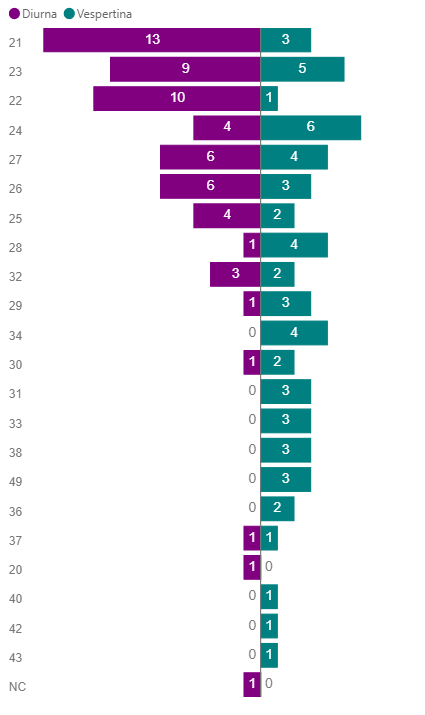
\includegraphics[width=0.55\textwidth]{figura1.png}
 \caption{Relación recuento edad por modalidad.}
 \label{figura 1}
 \source{elaboración propia.}
\end{figure}

Del total de test realizados ninguno de los evaluados obtuvo Abstracción Óptima. La \Cref{figura 2} muestra como el resultado No Abstracción predomina con un 61,1\%, sobre las otras evaluaciones, la sigue la Abstracción Satisfactoria con un 36,4\% y finalmente la Abstracción Buena con un 2,5\%. Esto quiere decir que el 97,4\% tienen un nivel de abstracción medio, lo que es muy preocupante, en especial el 61,1\% que no logró la habilidad cognitiva superior de abstraer.

\begin{figure}[htbp]
 \centering
 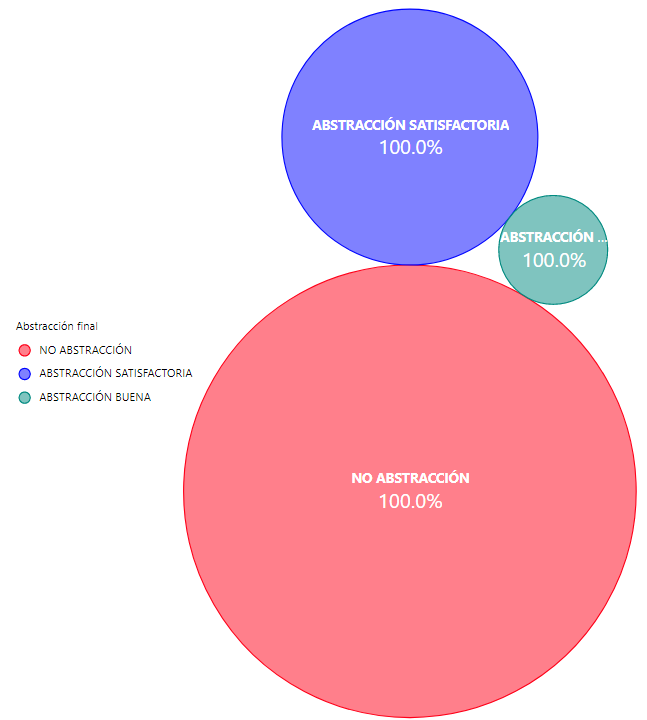
\includegraphics[width=0.75\textwidth]{figura2.png}
 \caption{Niveles de abstracción.}
 \label{figura 2}
 \source{elaboración propia.}
\end{figure}

De este análisis se puede observar en la \Cref{figura 3} que la relación de abstracción/modalidad sigue un patrón del 50\% para todas las categorías de abstracción. Por otro lado, en la \Cref{figura 4} y \Cref{figura 5}, se puede observar la relación abstracción/edad muestra que las categorías Abstracción Satisfactoria y No Abstracción se distribuyen homogéneamente en todas las edades y la Abstracción Buena no sigue una distribución homogénea, mostrando esta categoría para edades de 26, 29 y 40.

\begin{figure}[htbp]
 \centering
 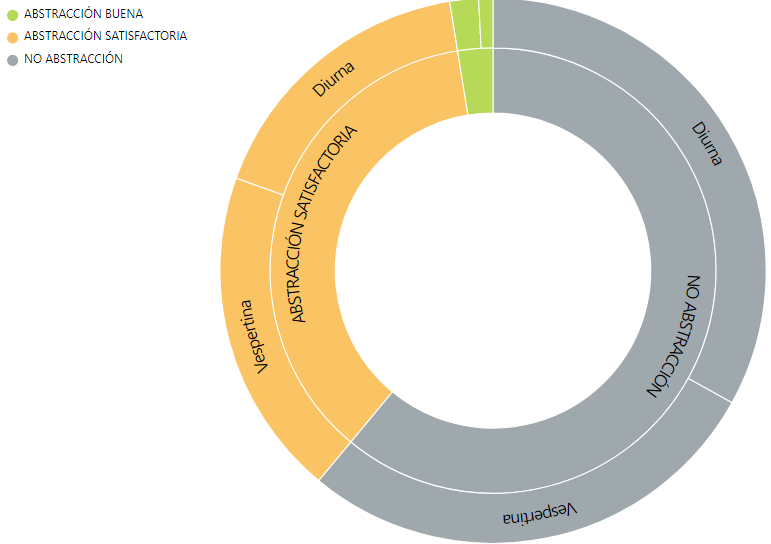
\includegraphics[width=0.75\textwidth]{figura3.png}
 \caption{Relación abstracción/modalidad}
 \label{figura 3}
 \source{elaboración propia.}
\end{figure}

\begin{figure}[htbp]
 \centering
 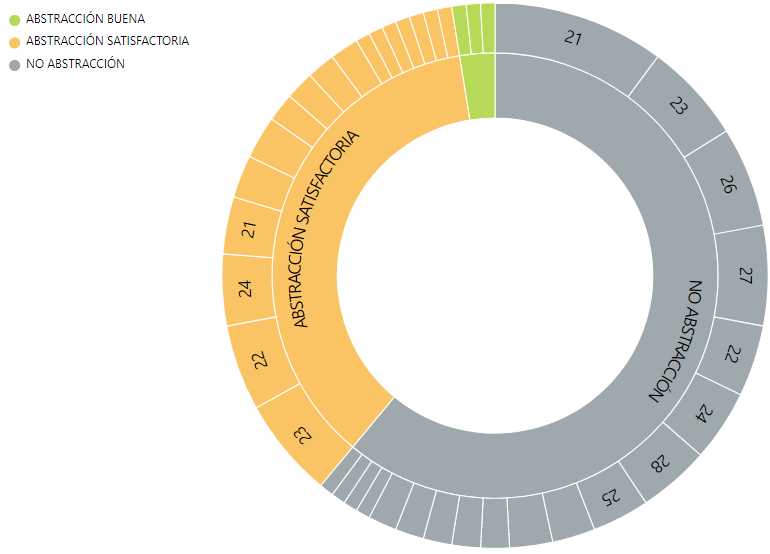
\includegraphics[width=0.75\textwidth]{figura4.png}
 \caption{Relación abstracción/edad.}
 \label{figura 4}
 \source{elaboración propia.}
\end{figure}

\begin{figure}[htbp]
 \centering
 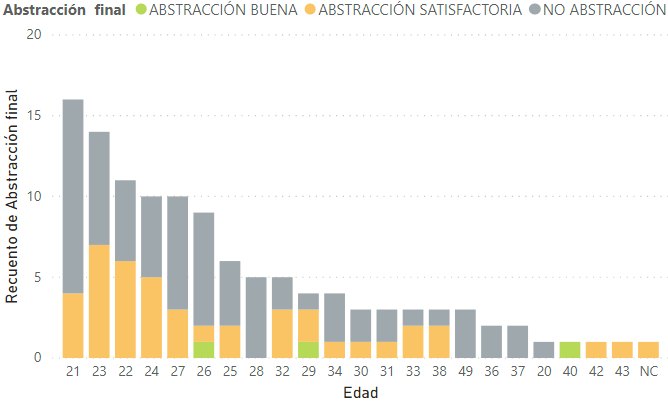
\includegraphics[width=0.75\textwidth]{figura5.png}
 \caption{Relación abstracción/edad.}
 \label{figura 5}
 \source{elaboración propia.}
\end{figure}

Del análisis se puede concluir que hay un problema con la abstracción que debe ser resuelto por medio de acciones de mejoras como cursos o capacitaciones, intervenciones focalizadas con el uso de la recursos digitales, por agrupaciones de los estudiantes que lo necesitan para no elevar su carga de estudio.

Esto es una solución factible si se piensa en estudiantes de primer o segundo semestre, donde un remedial puede ser una solución para semestres venideros. Sin embargo, como muestra la \Cref{figura 6}, el problema de la abstracción se acumula en el semestre 7, cuando el estudiante está a un semestre de terminar su carrera, y por lo tanto ya no es eficiente y efectivo activar una acción de mejora.

\begin{figure}[htbp]
 \centering
 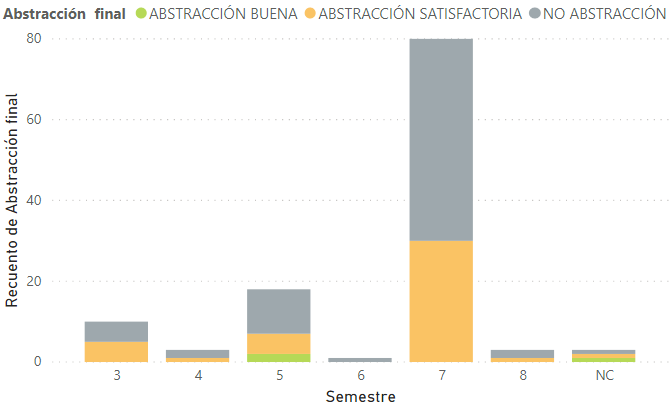
\includegraphics[width=0.75\textwidth]{figura6.png}
 \caption{Relación abstracción/semestre.}
 \label{figura 6}
 \source{elaboración propia.}
\end{figure}

Como se describió en párrafos anteriores, la intervención se puede hacer en los primeros semestres de la carrera para disminuir la baja abstracción en niveles superiores, pero sin asegurar que el estudiante no sea sobrecargado con la intervención.

Otro problema es que no adquirir esta habilidad cognitiva superior, puede llevar a la reprobación de las asignaturas, para ello, es necesario considerar habilidades inferiores como lo es la comparación, análisis y síntesis, entre otras \cite{beas2014, aravenagaete2021},  %(BEAS, SANTA CRUZ,  THOMSEN y UTRERAS,  2014; ARAVENA-GAETE, MARAMBIO, MARTIN y ROMERO, 2021)
como también utilizar recursos como el video juego, que hoy en tiempos de pandemia urge implementar la tecnología por parte de los profesores \cite{aznardiaz2017}. %(AZNAR-DÍAZ, RASO-SÁNCHEZ, HINOJO-LUCENA y ROMERO-DÍAZ DE LA GUARDIA, 2017). 
Entonces, lo ideal es encontrar este problema antes de que los estudiantes comiencen con las asignaturas regulares y que solo se intervenga a estudiantes con bajos niveles cognitivos.

\subsection{Análisis Predictivo}
Para el análisis predictivo se han preparado 6 experimentos programados en lenguaje R. \cite{chambers1992} %(CHAMBERS,  GENTLEMAN y  IHAKA, 1992)
Utilizando la base de datos del apartado anterior, se han diseñado 6 experimentos para detectar de forma temprana la falta de abstracción en los estudiantes. Como se explicó anteriormente, si este problema se detecta a inicios de cualquier ciclo académico, puede ser intervenido mediante acciones de mejora, como mitigación. En la actualidad los remediales se abordan en contingencia, de forma reactiva, y llegando muchas veces tarde.

Para los experimentos se utilizarán 6 algoritmos de máquina de aprendizaje supervisado que generarán los modelos de predicción: regresión logística (Logistic Regression), máquinas de soporte de vectores (support vector machine), Bayes ingenuo (Naive Bayes),  árbol de decisión (Decision Tree), bosque aleatorio (Random Forest) y k vecinos más cercanos (K nearest neighbors). Se compararán los distintos modelos para seleccionar el de mejor desempeño. En la página web de R-Project \cite{chambers1992}, %(CHAMBERS,  GENTLEMAN y  IHAKA, 1992)
se pueden encontrar las descripciones de todos estos algoritmos de máquinas de aprendizaje.

\subsection{Entrenamiento y pruebas de los modelos}
La base de datos abstracción es separada en un set de entrenamiento y otro para pruebas. El set de entrenamiento, como su nombre lo dice, estará a cargo de entrenar el modelo. El set de entrenamiento está compuesto por el 80\% de la base de datos de Abstracción. Así el set de prueba estará compuesto por el resto de registros de la base de datos de abstracción, un 20\% de los registros. El set de prueba servirá para evaluar el desempeño de los modelos de predicción.

La base de datos se divide en 8 variables de entrada, que se obtienen del test de abstracción realizado a los estudiantes, y 1 variable de salida que es la evaluación final del test de abstracción, la cual puede tener como resultado: No abstracción, Abstracción buena, Abstracción satisfactoria y Abstracción óptima, cuatro clases. La \Cref{figura7} muestra el modelo de predicción utilizado.

\begin{figure}[htbp]
 \centering
 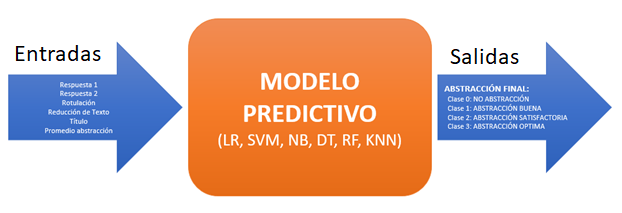
\includegraphics[width=0.75\textwidth]{figura7.png}
 \caption{Modelo Predictivo General con Entradas y Clases.}
 \label{figura7}
 \source{elaboración propia.}
\end{figure}

Para medir el desempeño de los modelos de predicción se utilizarán matrices de confusión y curvas ROC (receiver operating characteristic). La explicación de estas dos herramientas se puede encontrar \cite{chambers1992} %Chambers, Gentleman y  Ihaka (1992).

\subsection{Regresión Logística (Logistic Regression, LR)}
Los resultados obtenidos con el modelo de regresión logística se pueden observar en la Tabla 3, que describe la matriz de confusión de las predicciones del modelo comparados con el set de pruebas. Para una mejor visualización de la tabla llamaremos NA a la etiqueta No abstracción, AB a la etiqueta Abstracción buena, AS a la etiqueta Abstracción satisfactoria y AO a la etiqueta Abstracción óptima. La columna Prueba, hace referencia a los datos del set de Pruebas y al resultado de la misma. Las columnas Predicciones, hacen referencias a los resultados del modelo sobre las entradas del set de entrenamiento.

\begin{table}[htpb]
\centering
\caption{Matriz de Confusión Regresión Logística.}
\label{tab3}
\begin{tabular}{lllll}
\toprule 
 & \multicolumn{4}{l}{Predicciones}   \\ 
\cmidrule{2-5}
Pruebas        & NA      & AB       & AS       & AO
\\ 
\midrule
AB             & 0       & 0        & 0        & 0
\\ 
AS             & 1       & 10       & 0        & 0
\\
NA             & 0       & 12       & 0        & 0
\\
\bottomrule
\end{tabular}
\source{elaboración propia.}
\end{table}

De la \Cref{tab3} podemos concluir que 10 de 23 predicciones fueron erróneas, mientras que 13 de 23 predicciones acertaron. La \Cref{figura8}, muestra la curva ROC del modelo, y se observa que la curva es diagonal, lo que implica una modelo que ronda el 50\% de exactitud.

\begin{figure}[htbp]
 \centering
 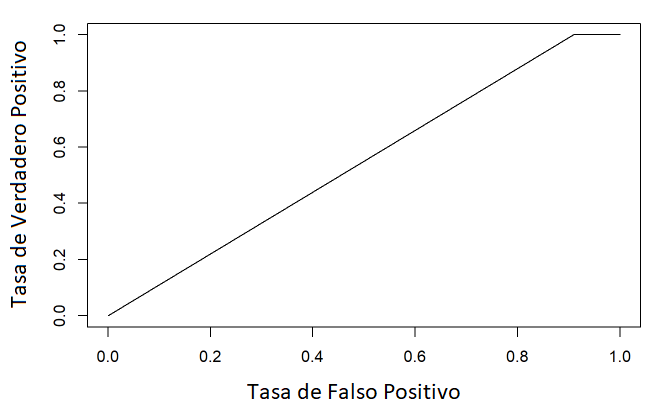
\includegraphics[width=0.55\textwidth]{figura8.png}
 \caption{Curvas ROC Regresión Logística.}
 \label{figura8}
 \source{elaboración propia.}
\end{figure}

Para confirmar estas afirmaciones, utilizaremos la \Cref{eq01}  
para encontrar la exactitud del modelo.


\begin{equation}\label{eq01}
    \textmd{Exactitud} = \frac{ VP + VN }{VP + FP + FN + VN}
\end{equation}
%(Ecuación 1)\\
Donde, 
TP son los resultados Verdaderos Positivos (True Positive),
TN son los resultados Verdaderos Negativos (True Negative),
FP son los resultados Falsos Positivos (False Positive) y 
FN son los resultados Falsos Negativos (False Negative).

Como resulto se obtiene una exactitud de 43,48\% para el modelo predictivo de regresión logística.

\subsection{Máquina Vectores de Soporte (Support Vector Machine, SVM)}
Los resultados obtenidos con el modelo de SVM  se puede observar en la \Cref{tab4}, que describe la matriz de confusión de las predicciones del modelo comparados con el set de pruebas.

\begin{table}[htpb]
\centering
\caption{Matriz de Confusión SVM.}
\label{tab4}
\begin{tabular}{lllll}
\toprule 
 & \multicolumn{4}{l}{Predicciones}   \\ 
\cmidrule{2-5}
Pruebas        & NA      & AB       & AS       & AO
\\ 
\midrule
AB             & 0       & 0        & 0        & 0
\\ 
AS             & 0       & 5        & 6        & 0
\\
NA             & 0       & 0        & 12       & 0
\\
\bottomrule
\end{tabular}
\source{elaboración propia.}
\end{table}

De la \Cref{tab4} podemos concluir que 6 de 23 predicciones fueron erróneas, mientras que 17 de 23 predicciones acertaron. La \Cref{figura9}, muestra la curva ROC del modelo, y se observa que la curva mejora, pues se acerca más a 1.

\begin{figure}[htbp]
 \centering
 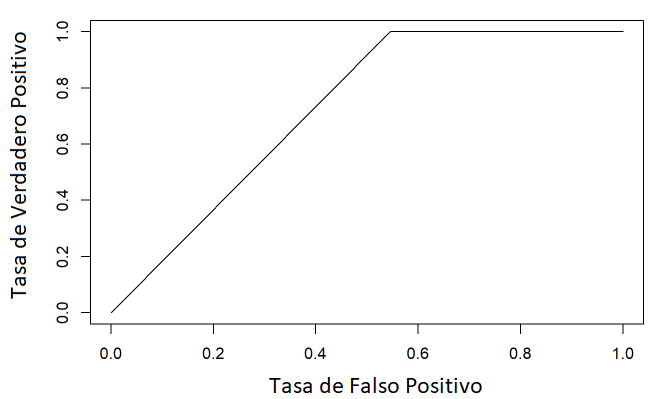
\includegraphics[width=0.55\textwidth]{figura9.png}
 \caption{Curvas ROC SVM.}
 \label{figura9}
 \source{elaboración propia.}
\end{figure}

Utilizando la \Cref{eq01} se obtiene una exactitud de 73,91\% para el modelo SVM. Que mejora 30, 43\% sobre el modelo SVM.

\subsection{Árbol de Decisión (Decision Tree, DT)}
Los resultados obtenidos con el modelo de DT  se puede observar en la \Cref{tab5}, que describe la matriz de confusión de las predicciones del modelo comparados con el set de pruebas.

\begin{table}[htpb]
\centering
\caption{Matriz de Confusión DT.}
\label{tab5}
\begin{tabular}{lllll}
\toprule 
 & \multicolumn{4}{l}{Predicciones}   \\ 
\cmidrule{2-5} 
Pruebas        & NA      & AB       & AS       & AO
\\ 
\midrule
AB             & 0       & 0        & 0        & 0
\\ 
AS             & 0       & 11       & 0        & 0
\\
NA             & 0       & 0        & 12       & 0
\\
\bottomrule
\end{tabular}
\source{elaboración propia.}
\end{table}

De la \Cref{tab5} podemos concluir que 0 de 23 predicciones fueron erróneas, mientras que 23 de 23 predicciones acertaron. La \Cref{figura10}, muestra la curva ROC del modelo, y se observa que la curva es una constante 1 en el eje horizontal, lo que implica un 100\% de predicciones realizadas correctamente.

\begin{figure}[htbp]
 \centering
 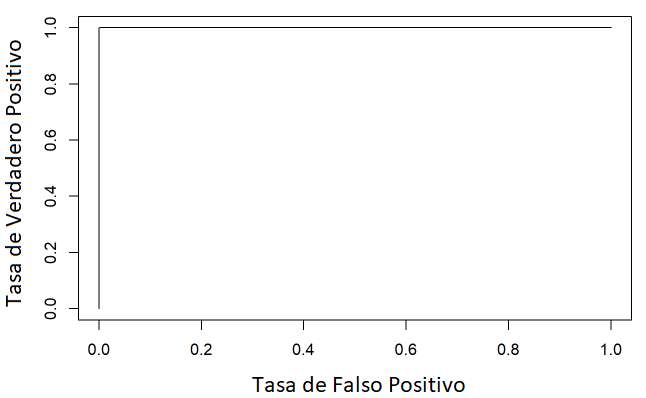
\includegraphics[width=0.55\textwidth]{figura10.png}
 \caption{Curvas ROC DT.}
 \label{figura10}
 \source{elaboración propia.}
\end{figure}

Utilizando la \Cref{eq01} se obtiene una exactitud de 100,00\% para el modelo DT.

\subsection{Naïve Bayes, NB}
Los resultados obtenidos con el modelo de NB  se pueden observar en la Tabla 6, que describe la matriz de confusión de las predicciones del modelo comparados con el set de pruebas.

\begin{table}[htpb]
\centering
\caption{Matriz de Confusión NB.}
\label{tab6}
\begin{tabular}{lllll}
\toprule 
  & \multicolumn{4}{l}{Predicciones}   \\ 
\cmidrule{2-5}
Pruebas        & NA      & AB       & AS       & AO
\\ 
\midrule
AB             & 0       & 0        & 0        & 0
\\ 
AS             & 1       & 10       & 0        & 0
\\
NA             & 0       & 0        & 12       & 0
\\
\bottomrule
\end{tabular}
\source{elaboración propia.}
\end{table}

De la \Cref{tab6} podemos concluir que 1 de 23 predicciones fueron erróneas, mientras que 22 de 23 predicciones acertaron. La \Cref{figura11}, muestra la curva ROC del modelo, y se observa que la curva es tangencial a 1.

\begin{figure}[htbp]
 \centering
 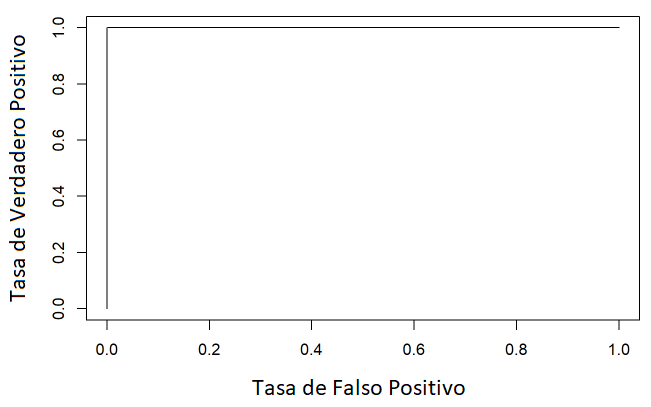
\includegraphics[width=0.55\textwidth]{figura11.png}
 \caption{Curvas ROC NB.}
 \label{figura11}
 \source{elaboración propia.}
\end{figure}

Utilizando la \Cref{eq01} se obtiene una exactitud de 95,65\% para el modelo NB, bajando 4,35\% respecto al modelo DT.

\subsection{Bosque aleatorio (Ramdom Forest; RF)}
Los resultados obtenidos con el modelo de RF  se pueden observar en la \Cref{tab7}, que describe la matriz de confusión de las predicciones del modelo comparados con el set de pruebas.

\begin{table}[htpb]
\centering
\caption{Matriz de Confusión RF.}
\label{tab7}
\begin{tabular}{lllll}
\toprule 
 & \multicolumn{4}{l}{Predicciones}   \\ 
\cmidrule{2-5}
Pruebas        & NA      & AB       & AS       & AO
\\ 
\midrule
AB             & 0       & 0        & 0        & 0
\\ 
AS             & 0       & 11       & 0        & 0
\\
NA             & 0       & 0        & 12       & 0
\\
\bottomrule
\end{tabular}
\source{elaboración propia.}
\end{table}

De la \Cref{tab7} podemos concluir que 1 de 23 predicciones fueron erróneas, mientras que 22 de 23 predicciones acertaron. La \Cref{figura12}, muestra la curva ROC del modelo, se observa que la curva es una constante 1 en el eje horizontal, lo que implica un 100\% de predicciones realizadas correctamente.

\begin{figure}[htbp]
 \centering
 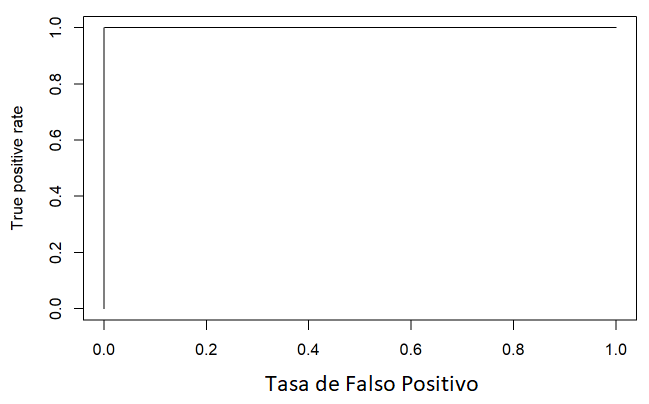
\includegraphics[width=0.55\textwidth]{figura12.png}
 \caption{Curvas ROC RF.}
 \label{figura12}
 \source{elaboración propia.}
\end{figure}

Utilizando la \Cref{eq01} se obtiene una exactitud de 100,00\% para el modelo RF, igualando al modelo DT.

\subsection{K Vecinos más Cercanos (K Nearest Neighbors; KNN)}
Los resultados obtenidos con el modelo de KNN  se puede observar en la \Cref{tab8}, que describe la matriz de confusión de las predicciones del modelo comparados con el set de pruebas.

\begin{table}[htpb]
\centering
\caption{Matriz de Confusión KNN.}
\label{tab8}
\begin{tabular}{lllll}
\toprule 
 & \multicolumn{4}{l}{Predicciones}   \\ 
\cmidrule{2-5}
Pruebas        & NA      & AB       & AS       & AO
\\ 
\midrule
AB             & 0       & 0        & 0        & 0
\\ 
AS             & 0       & 6        & 5        & 0
\\
NA             & 0       & 0        & 12       & 0
\\
\bottomrule
\end{tabular}
\source{elaboración propia.}
\end{table}

De la \Cref{tab8},  podemos concluir que 6 de 23 predicciones fueron erróneas, mientras que 17 de 23 predicciones acertaron. La \Cref{figura13}, muestra la curva ROC del modelo, y se observa que la curva se comporta como la curva del modelo SVM.

\begin{figure}[htbp]
 \centering
 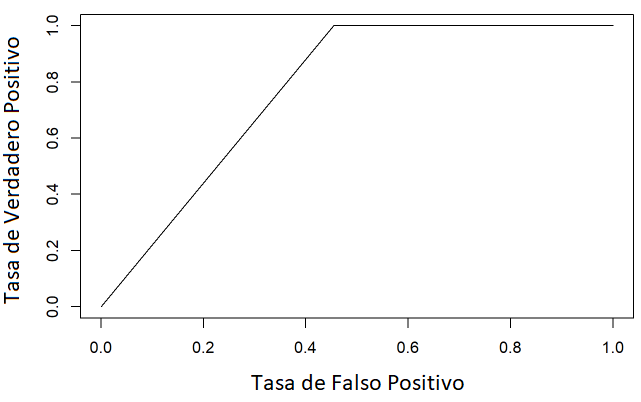
\includegraphics[width=0.55\textwidth]{figura13.png}
 \caption{Curvas ROC KNN.}
 \label{figura13}
 \source{elaboración propia.}
\end{figure}

Utilizando la \Cref{eq01} se obtiene una exactitud de 73,91\% para el modelo KNN.

\subsection{Discusión y conclusiones}
En la tabla 9, se pueden observar los resultados obtenidos para la base de datos de registros utilizados para probar los modelos creados con la base de datos de registros de entrenamiento.

\begin{table}[htpb]
\centering
\caption{Curvas ROC KNN.}
\label{tab9}
\begin{tabular}{lllll}
\toprule 
 & \multicolumn{3}{l}{Predicciones}  & \\ 
\cmidrule{2-4}
Modelo     & TP+TN      & FP+FN     & Accuracy     & Elección Modelo
\\ 
\midrule
LR         & 13         & 10       & 43,48\%       & No
\\ 
SVM        & 17         & 6        & 73,91\%       & No
\\
DT         & 23         & 0        & 100,00\%      & Si
\\
NB         & 22         & 1        & 95,65\%       & No
\\
RF         & 23         & 0        & 100,00\%      & Si
\\
KNN        & 17         & 6        & 73,91\%       & No
\\
\bottomrule
\end{tabular}
\source{elaboración propia.}
\end{table}

El modelo con menor rendimiento es LR con una exactitud del 43,48\%. Lo que implica que en la mitad de los casos cometería errores en la predicción de la alerta temprana. Comprado con los otros modelos, podemos sin dudas descartarlo.

Luego podemos observar que el modelo SVM y KNN, poseen una exactitud de 73,91\%. Si bien es un buen resultado, cuando aumenta el número de casos que se analizan, aumenta el número de errores que se cometen. En la muestra solo se ven 6 errores, pero si esa muestra aumenta a 100, implica que pasan a ser 26 errores. Es por esta razón que se descarta.

El modelo NB muestra una exactitud del 95,65\%, que es un excelente resultado. Ya este modelo puede ser una elección satisfactoria para la detección temprana de la falta de abstracción. Sin embargo, se descarta porque hay dos modelos, DT y RF, que tienen un rendimiento mejor, llegando a una exactitud del 100\%.

Los resultados de los últimos 3 modelos nombrados (NB, DT y RF) nos llevan a concluir que se puede detectar tempranamente la falta de abstracción de los estudiantes, utilizando las variables de entrada provenientes del test. Esto implica que se pueden diseñar e implementar acciones de mejora a esta problemática, antes que los estudiantes afronten asignaturas donde se hace necesario llegar con este tipo de habilidades cognitivas superiores.  

Bajo este desafío, se propone un análisis proyectivo, de detección temprana de estudiantes con baja abstracción, utilizando modelos de máquina de aprendizaje supervisado y la utilización del video juego para el desarrollo cognitivo superior.

Los investigadores apuestan por los videojuegos de acción en relación al desarrollo de la actividad cognitiva. “Son juegos que requieren que los jugadores activen los reflejos y movimientos rápidos, demandando un alto seguimiento de varios elementos a la vez y generando una gran cantidad de información que debe ser procesada, mientras se toman decisiones en una fracción de segundo” \cite[p. 29]{moscardi2018}. %(MOSCARDI, 2018, p. 29).

%%%%%%%%%%%%%%%%%%%%%%%%%%%%%%%%%%%%%%%%%%%%%%%%%%%%%%%%%
%%%%%%%%%%%%%%%%%%%%%%%%%%%%%%%%%%%%%%%%%%%%%%%%%%%%%%%%%
%%%%%%%%% FIM REMOVER %%%%%%%%%%%%%%%%%%%%%%%%%%%%%%%%%%%
%%%%%%%%%%%%%%%%%%%%%%%%%%%%%%%%%%%%%%%%%%%%%%%%%%%%%%%%%
%%%%%%%%%%%%%%%%%%%%%%%%%%%%%%%%%%%%%%%%%%%%%%%%%%%%%%%%%


\printbibliography\label{sec-bib}
% if the text is not in Portuguese, it might be necessary to use the code below instead to print the correct ABNT abbreviations [s.n.], [s.l.] 
%\begin{portuguese}
%\printbibliography[title={Bibliography}]
%\end{portuguese}



\end{document}
